% 
% sudo apt install texlive-fonts-extra
% may be requered sudo apt install cm-super
% 
% compile with pdflatex
%

\documentclass[hyperref={pdfpagelabels=false}]{beamer}
\usepackage{amssymb,amsmath,cancel,cite,color,cmap,float,graphicx,lmodern,listings,
  multirow,pifont,pgfplots,txfonts,tikz,wrapfig,xcolor,yfonts}

\hypersetup{
    colorlinks=true,
    linkcolor=white,
    filecolor=magenta,
    urlcolor=blue,
}

\usepackage{paratype}
\renewcommand*\familydefault{\sfdefault}
\usepackage[T1, T2A]{fontenc}
\usepackage[utf8]{inputenc}
\usepackage[english,russian]{babel}
\usepackage{hyperref}

% some weird help from tex compiler
\pgfplotsset{compat=1.15}

\usetikzlibrary{arrows,automata,positioning,shapes,shapes.multipart}
\usetheme{Copenhagen}

\setbeamertemplate{navigation symbols}{}
%\addtobeamertemplate{number}{}{%
%    \usebeamerfont{footline}%
%    \usebeamercolor[black]{footline}%
%    \hspace{1em}%
%    \insertframenumber%/\inserttotalframenumber
%}

%\expandafter\def\expandafter\insertshorttitle\expandafter{%
%  \insertshorttitle\hfill%
%  \insertframenumber}
\newcommand*\circled[1]{\tikz[baseline=(char.base)]{
    \node[shape=circle,draw,inner sep=2pt] (char) {#1};}}
\addtobeamertemplate{navigation symbols}{}{
  \usebeamerfont{footline}
  \fontsize{12pt}{12}\selectfont
  \usebeamercolor[black]{footline}
  \hspace{1em}
  \circled{${\insertframenumber}$}
}
%\textswab
\setbeamertemplate{frametitle}[default][center]


\definecolor{codegreen}{rgb}{0,0.6,0}
\definecolor{codegray}{rgb}{0.5,0.5,0.5}
\definecolor{codepurple}{rgb}{0.58,0,0.82}
\definecolor{backcolour}{rgb}{0.95,0.95,0.92}

\lstdefinestyle{mystyle}{
    backgroundcolor=\color{backcolour},   
    commentstyle=\color{codegreen},
    keywordstyle=\color{magenta},
    numberstyle=\tiny\color{codegray},
    stringstyle=\color{codepurple},
    basicstyle=\ttfamily\footnotesize,
    breakatwhitespace=false,         
    breaklines=true,                 
    captionpos=b,                    
    keepspaces=true,                 
    numbers=left,                    
    numbersep=5pt,                  
    showspaces=false,                
    showstringspaces=false,
    showtabs=false,                  
    tabsize=2
}

\lstdefinelanguage{my_pseudo} {
	morekeywords={function, for, return, let, in},
	sensitive=false,
	morecomment=[l]{//},
	morecomment=[s]{/*}{*/},
	morestring=[b]",
}

\lstset{style=mystyle}
\lstset{language=my_pseudo}



\begin{document}
  
\title[Специализация алгоритма Витерби]{Специализация алгоритма Витерби скрытой марковской моделью}  
\author[И. Тюляндин]{Иван Тюляндин\\%
Научный руководитель: к.\,ф.-м.\,н., доцент кафедры информатики С.\,В. Григорьев\\%
Консультант: к.\,ф.-м.\,н., старший преподаватель кафедры современного программирования Д.\,А.\,Березун\\%
} 
\date{19 декабря 2020} 
{
\setbeamertemplate{navigation symbols}{}
\frame[noframenumbering,plain]{
\maketitle
} 
}


\begin{frame}{Задача гомологичности}
\begin{block}{Задача гомологичности}
	Поиск эволюционных предков у исследуемого протеина и изученных протеинов
	\begin{itemize}
		\item символьные последовательности аминокислот
		\item вероятности сходства последовательностей
	\end{itemize}
\end{block}
\end{frame} 


\begin{frame}{Скрытые марковские модели}
\begin{block}{Скрытая марковская модель}
\begin{itemize}
	\item St[N] — множество состояний
	\item Obs[K] — множество наблюдений
	\item Pr\_b[N] — вероятности состояний быть начальными
	\item Tr[N][N] — вероятности переходов между состояниями
	\item Em[N][K] — вероятности наблюдений в состояниях
\end{itemize}
\end{block}
\end{frame}


\begin{frame}[fragile]{Aлгоритм Витерби}
\begin{block}{Алгоритм Витерби}
\begin{lstlisting}[escapeinside={(*}{*)}]
function Viterbi(St, Obs, Pr_b, Tr, Em, O)
	T = length(O)
	Dp[T][N]

	for j = 1..N
		Dp[1][j] = Pr_b[j] * Em[j][O[1]]
	
	for i = 2..T
		for j = 1..N
			Dp[i][j] = 
					(*$\max_{x = 1..N}$*)(Dp[i-1][x] * Tr[x][j] * Em[j][O[i]])

	return Dp[T]
\end{lstlisting}
\end{block}
\end{frame}


\begin{frame}{Специализация}
\begin{figure}
	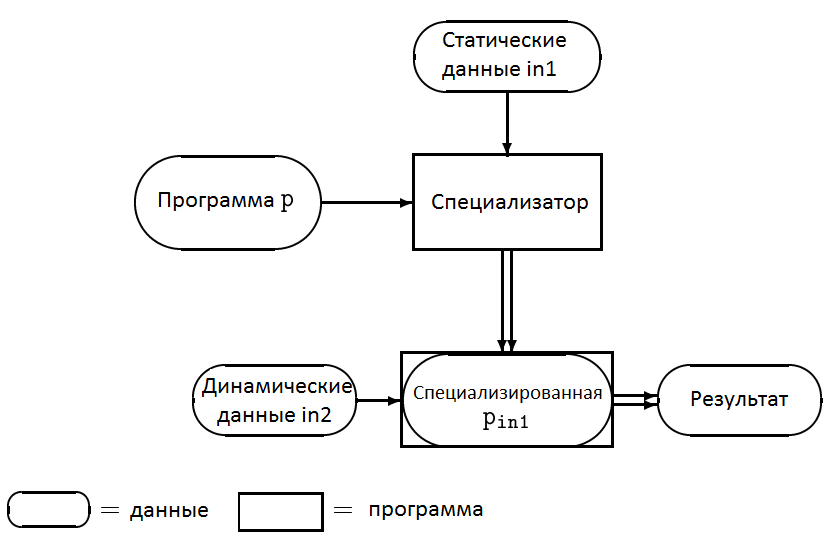
\includegraphics[scale=0.45]{spec.png}
	\caption{Специализация}
\end{figure}
\end{frame} 


\begin{frame}{Цель работы}
\begin{block}{Цель}
Исследовать применимость специализации алгоритма Витерби
\end{block}
\vfill
\begin{figure}
	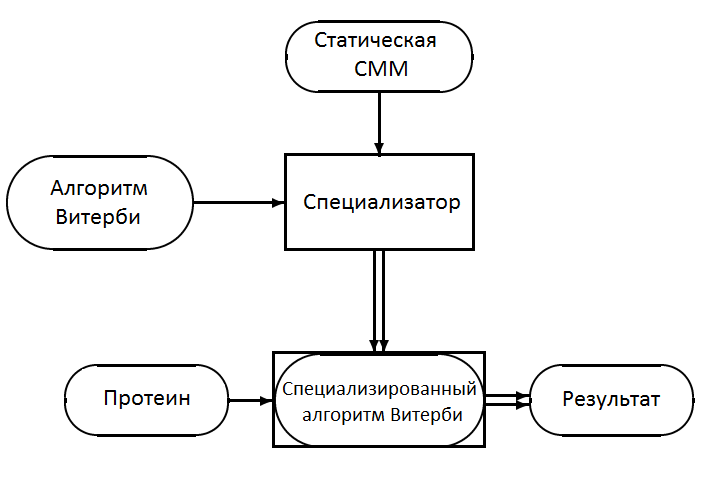
\includegraphics[scale=0.40]{spec_Viterbi.png}
\end{figure}
\end{frame}


%\begin{frame}{Поставленные задачи}
%\begin{itemize}
%	\item Сделать обзор предметной области и существующих решений 
%		задачи гомологичности
%	\vfill
%	\item Реализовать неспециализированную версию алгоритма Витерби
%	\vfill
%	\item Написать специализатор алгоритма Витерби на СММ
%	\vfill
%	\item Провести сравнительный анализ производительности
%\end{itemize}
%\end{frame}


\begin{frame}{Специализация GPGPU}
\begin{block}{Специализация GPGPU}
	Идея: перенос статических данных в код уменьшит промахи 
	кэша данных на GPGPU
\end{block}
\vfill
Специализированный наивный поиск подстроки в строке быстрее в 8 раз. 
Статья  А. Тюрина, С. Григорьева и Д. Березуна \href{https://www.researchgate.net/publication/339368918_Optimizing_GPU_programs_by_partial_evaluation}{Optimizing GPU programs by partial evaluation}
\vfill
Стандарт OpenCL
\vfill
Генерация ядер с распространением констант
\end{frame}


\begin{frame}{Специализация GPGPU: замеры}
    \begin{tikzpicture}
        \begin{axis}[%
	        title={OpenCL, NVIDIA GeForce GTX 1030},
            axis x line=bottom,
            axis y line=left,
            xlabel={Кол-во состояний СММ},
            ylabel={Время, мсек},
            ymin=1500, ymax=2600,
            legend pos=south east]
            \addplot[mark=square,red,thick] table[x=states,y=non_spec] {OpenCL_bench.dat};
            \addplot[mark=square,blue,thick] table[x=states,y=spec] {OpenCL_bench.dat};
            \legend{Обыч., Спец.}
        \end{axis}
	\end{tikzpicture}
\end{frame}


\begin{frame}{Специализация алгоритма линейной алгебры}
\begin{block}{Специализация алгоритма линейной алгебры}
	Идея: выразить алгоритм Витерби через матричные операции, 
		а затем предпосчитать часть операций
\end{block}
\vfill
	Статья E. Theodosis и P. Maragos: \href{http://cvsp.cs.ntua.gr/publications/confr/2018_TheodosisMaragos_AnalysisViterbi-TropicalAlgebraGeometry_SPAWC.pdf}
	{Analysis of the Viterbi Algorithm Using 
	Tropical Algebra and Geometry}
\vfill
	Можно сократить количество умножений матриц
\vfill
	Разреженные матрицы в СММ
\vfill
	Использование библиотеки SuiteSparse:GraphBLAS
\end{frame}


\begin{frame}{Специализация алгоритма линейной алгебры: замеры}
	    \begin{tikzpicture}
        \begin{axis}[%
	        title={SuiteSparse:GraphBLAS, Intel Core i7-4790},
            axis x line=bottom,
            axis y line=left,
            xlabel={Кол-во состояний СММ},
            ylabel={Время, мсек},
            legend pos=south east]
            \addplot[mark=square,red,thick] table[x=states,y=non_spec] {GraphBLAS_bench.dat};
            \addplot[mark=square,blue,thick] table[x=states,y=spec] {GraphBLAS_bench.dat};
            \legend{Обыч., Спец.}
        \end{axis}
	\end{tikzpicture}
\end{frame}


\begin{frame}{Различие определений СММ}
	HMMer и CUDAMPF --- существующие решения
	с использованием нестандартного определения СММ
\vfill
	Реализованные специализаторы используют разные 
	определения СММ
\vfill
	Необходим конвертер для проведения эксперимента
\end{frame}


\begin{frame}{Текущие результаты}
\begin{itemize}
	\item Сделан обзор предметной области
	\item Реализованы две версии неспециализированного 
	алгоритма Витерби
	\item Написаны два специализатора
	\item (TODO) Конвертер и сравнение специализаторов
\end{itemize}
\vfill
Код доступен по ссылкам:
\begin{itemize}
	\item OpenCL\\
	\href{https://github.com/IvanTyulyandin/HMM_FASTA_Viterbi}{github.com/IvanTyulyandin/HMM\_FASTA\_Viterbi}
	\item SuiteSparse:GraphBLAS\\
	\href{https://github.com/IvanTyulyandin/Lin_alg_Viterbi}{github.com/IvanTyulyandin/Lin\_alg\_Viterbi}
\end{itemize}
\end{frame}

% Опорные слайды
\begin{frame}{Матричный алгоритм Витерби}
	Вероятности в отрицательные логарифмы, MIN\_PLUS операции
\vfill
\[
  P(obs) =
  \begin{bmatrix}
    p_{1}(obs) & \hdots & +\infty \\
    \vdots & \ddots & \vdots\\
    +\infty & \hdots & p_{n}(obs)
  \end{bmatrix}
\]
\vfill
Начало алгоритма Витерби\\
\[Probs_{0} = P(Obs[0]) * Pr_b\]
\vfill
Шаг алгоритма Витерби\\
\[Probs_{t} = P(Obs[t]) * Tr^{T} * Probs_{t - 1}\]
\end{frame}


\begin{frame}{}
\begin{block}{Замеры}
\begin{itemize}
	\item Ubuntu 20.04, 32 Гб RAM, Intel Core i7-4790 3.60 GHz, NVIDIA GeForce GTX 1030
	\item OpenCL 1.2, SuiteSparse:GraphBLAS 3.3.3
	\item СММ с одинаковым количеством состояний и переходов
	\item 3 последовательности по 7000 наблюдений
	\item лучшее время из 3 запусков
\end{itemize}
\end{block}
\vfill
\begin{block}{Тестирование}
\begin{itemize}
	\item корректность считывания форматов
	\item ожидаемые ответы на заранее заданных данных
	\item сохранение семантики после специализации
	\item утечки памяти (Valgrind)
\end{itemize}
\end{block}
\end{frame}

\end{document}
